\newcommand{\spuli}{\text{spüli}}
\newcommand{\wasser}{\text{wasser}}
\subsection{Aufstieg von Luftblasen}
	\subsubsection{Dichte des Spülmittels}
		Nach dem Archimedischen Prinzip ist die Auftriebskraft, die die Flasche ins Wasser hält, gleich die Gewicht des verdrängten Wasser. Somit gilt:
		\begin{equation}
			F_A = \rho_\wasser V_\wasser g
		\end{equation}
		Da die Flasche im Wasser schwimmt, also ist die Flasche im Gleichgewicht und es gilt:
		\begin{align}
			F_G &= F_A \\
			\rho_\spuli V_\spuli \cancel{g} &= \rho_\wasser V_\wasser \cancel{g} \\
			\rho_\spuli &= \rho_\wasser \frac{V_\wasser}{V_\spuli}
		\end{align}
		Dabei ist die Volumen des verdrängtes Wasser als $V_\wasser = \SI{650(50)}{\centi\meter\cubed}$.

		\begin{wrapfigure}{o}{0.4\textwidth}
			\centering
			\vspace{-1em}
			\captionsetup{width=0.4\textwidth, justification=centering}
			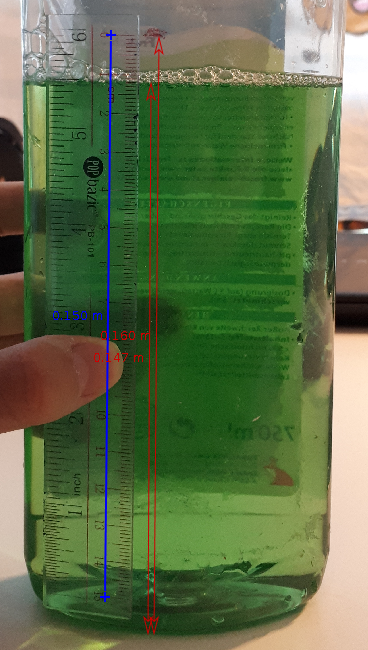
\includegraphics[width=0.25\textwidth]{tv1-dichte-auswertung.png}
			\caption{Messungen der Höhe des Wasserpegels in \tracker{}}
			\vspace{-1em}
		\end{wrapfigure}
		Wir nehmen an, dass der Flasche die Querschnittsfläche für den unteren Teil überall gleich ist, somit ist das Volumen proportional zur Höhe und wir erhalten:
		\begin{align}
			\rho_\spuli &= \rho_\wasser \frac{h_\wasser}{h_\spuli}
		\end{align}
		Aus \tracker{} haben wir als Messwerten:
		\begin{center}
			\begin{tabular}{llr}
				\toprule
				Höhe des Wasserpegels & $h_\wasser$ & \SI{}
				\bottomrule
			\end{tabular}
		\end{center}



	\subsubsection{Viskosität des warmen Spülmittels}
	\subsubsection{Viskosität des kalten Spülmittels}
	\subsubsection{Diskussion}